\documentclass[twoside,twocolumn]{article}
\renewcommand\thesection{\roman{section}} 
\renewcommand\thesubsection{\Alph{subsection}}
\renewcommand\thesubsubsection{\arabic{subsubsection}}
\usepackage{amsmath}
\usepackage{algorithm}  
\usepackage{algorithmic}  
\usepackage{amsmath}  
\renewcommand{\algorithmicrequire}{\textbf{Input:}}  % Use Input in the format of Algorithm  
\renewcommand{\algorithmicensure}{\textbf{Output:}} % Use Output in the format of Algorithm 
\usepackage{amssymb}
\usepackage{subfigure}
\usepackage[english]{babel}
\usepackage{graphicx}
\usepackage{titlesec}
\usepackage{indentfirst}
\setlength{\parindent}{2em}
\usepackage[hmarginratio=1:1,top=32mm,columnsep=15pt]{geometry}
\titleformat{\section}[block]{\large\scshape\centering}{\thesection.}{1em}{} % Change the look of the section titles
\titleformat{\subsection}[block]{\large}{\thesubsection.}{1em}{} % Change the look of the section titles
\title{Power Consumption and Delay}
\author{Wei Xiang}  % no author
\begin{document}
\maketitle
%\clearpage
\section{Introduction}
\section{Related Work}
\section{SYSTEM MODEL AND PROBLEM FORMULATION}
In this section,we give an overview of our approach toward  delay and power consumption. As shown in figure 1,the system architecture that we consider comprises : a set of Roadside Units(RSUs),a set of fog devices and a set of cloud servers.The RSUs receive requests from users and send them to a set N of fog devices through a Local Area Network(LAN),which act as users' interfaces. Fog nodes can process some delay-sensitive,light-level requests and forward other delay-tolerant requests to a set N of cloud servers through a Wide Area Network(WAN). Each cloud server hosts a lot of homogeneous computing machines.Since the WAN covers a large geographical area from the fog to the cloud, the transmission delay can not be omitted[compared to the LAN].The communication delay and the bandwidth limitation should be taken into account. Moreover,the computation delay of fog node or cloud node also should be considered. In addition, the power consumption and delay are also considered in our proposal system. Hence,we mainly consider consumption and delay in four components(i.e.cloud layer,fog layer, transmission in WAN, transmission in VANET). The used notation is summarized in table I.
\begin{figure}[h]
\centering
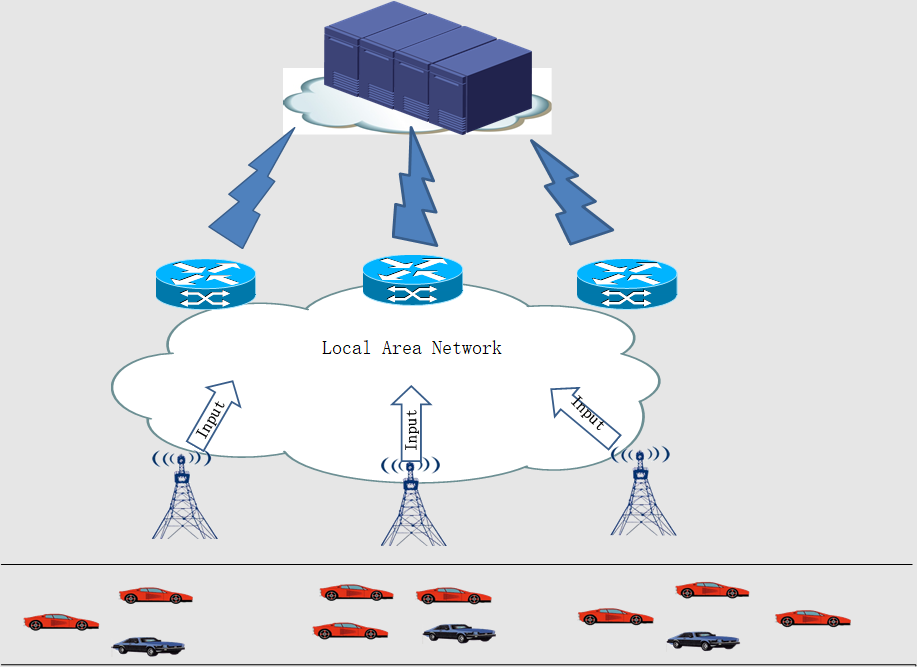
\includegraphics[scale=0.4]{4.png}
\caption{Overall architecture of a fog-cloud computing system}
\label{fig:label}
\end{figure}

\begin{table}[h]
	\centering
	\begin{tabular}{p{1cm}p{5cm}}
	\hline
	Symbol & Definition \\\hline
	$i,N,\mathcal{N}$ & index, number, set of fog devices\\
	$j,M,\mathcal{M}$ & index, number, set of cloud devices\\
	$r,R,\mathcal{R}$ & index, number, set of RSUs\\
	$u,U,\mathcal{U}$ & index, number, set of vehicles\\
	$\lambda_{ij}$    & traffic rate dispatched from fog device $i$ to cloud server $j$\\
	$y_j$             & workload assigned to cloud server $j$\\
	$f_i$	          & CPU frequency of fog device $i$ \\
	$L$               & total input from all RSUs\\
	$X$               & workload allocated for fog computing\\
	$Y$               & workload allocated for cloud server\\
	$P$               & power consumption\\
	$D$               & delay\\
	$s_j$             & the remaining requests on cloud server from last interval $j$\\
	$s_i$             & the remaining requests on fog device  from last interval $i$\\
	$v_i$             & service rate for fog device $i$\\
	$f_j$             & machine CPU frequency at cloud server $j$\\
	$\sigma_j$        & on/off state of cloud server $j$\\
	$b_{ur}$               & $2 \times 1$ dimension matrix\\      
	$n_j$             & machine number in cloud server $j$\\
	$d_{i,j}$         & communication delay from fog device $i$ to cloud server $j$\\\hline
	\end{tabular}
	\caption{Symbols}
\end{table}


\subsection{System Model}
We concern to minimize the consumption with an guaranteed delay in our system model. So, we are mainly concerned about the following parts.

\textit{1) Power Consumption of Fog Device:} The computation power consumption of fog device \textit{i} can be calculated by a function of the CPU frequency $f_i$.The function must be a monotonic increasing and strictly convex function. The piece-wise linear function and quadratic function are two candidates. Generally speaking, the power consumption functions of the fog computing device have a number of different forms as long as the functions satisfy the following constraints: \textit{a):}  the function result always increases as the CPU frequency increases. \textit{b):} the marginal power consumption for each fog device is increasing.For simplicity but without loss of generality,the power consumption $p_i^{fog} $ of device $i$ is defined as follows.
$$ p_i^{fog} \triangleq a_if_i^2+b_if_i+c_i $$
where $f_i$ is the CPU frequency of fog device $i$ and $a_i,b_i,c_i$ are non-negative,pre-determined parameters. 

\textit{2) Communication Delay of Fog Device:} We assume that it is a queueing system for the fog device to process requests. For the device $i$ with traffic arrival rate $x_i$ and service rate $v_i$, the computation delay $D_i^{fog}$ which includes waiting time and service time is 
$$ D_i^{fog} \triangleq \frac{1}{v_i-x_i} .$$

\textit{3) Power Consumption of Cloud Server:} As mentioned before, each cloud server hosts numerous homogeneous computing machines. We simply assume that the CPU frequencies of these machines are equal in a cloud server. The number of turned-on machines in cloud server $j$ is denoted by $n_j$ In this situation, the power consumption of cloud server $j$ can be expressed as the product of the turned-on machine consumption value and the number of machines in server $j$. We approximate the power consumption value of each machine in server $j$ by a function of CPU frequency $f_j$:$P^{mh} = A_jf_j^p+B_j$, where $A_j$ and $B_j$ are positive constants, and $p$ is in the range of 2.5 to 3. 

At a specific moment, some cloud servers are powered on for computation service whereas more server are powered off for energy saving especially when the workload decreased. We use a binary variable $\sigma_j$ denote the on/off state of cloud server $j$. Specifically, 0 indicates that the server is off and 1 means on. Hence, the power consumption $P_j^{cloud}$ of the cloud server $j$ can be calculated by multiplying the number of turned-on machines and each machine power consumption value.
$$P_j^{cloud} = \sigma_jn_j\left(A_jf_j^p+B_j\right)$$

\textit{4) Communication Delay of Cloud Server:} The delay of cloud server can be obtained by $D_i^{cloud} = t_{queue}+t_{service}$. We model the system as a queueing network, and the cloud can be modeled as $M/M/n$ queue. According to queueing theory, average queueing time $t_{queue}$ is $\frac{C(n,\lambda/\mu)}{n\mu-\lambda}$,where n is the number of turned-on machines,$\lambda$ and $\mu$ respectively indicate traffic arrival rate and service rate. We assume each machine in cloud server $j$ has the same service rate $\mu_{j}$. Thus, the $\mu_j$ can be converted to $f_j/K$,where k is average cycles per request.(cycles/request). According to the definition of service rate, the service time $t_{service}$ is the reciprocal of service rate $\mu$. Thus, the total computation delay of cloud server is given by
$$D_j^{cloud} \triangleq \sigma_j\left[\frac{C\left(n_j,y_jK/f_j\right)}{n_jf_j/K-y_j} + \frac{K}{f_j}\right].$$

\textit{5) Communication Delay of Transmission:}
Communication delay of dispatch: We use $d_{ij}$ to record the transmission delay from fog device $i$ to the cloud server $j$. Let the binary variable $\lambda_{ij}$ denote the traffic rate dispatched from the fog device $i$ to the cloud server $j$. The communication delay of dispatch is 
$$ D_{ij}^{dis} \triangleq d_{ij}\lambda_{ij} .$$
Communication delay of VANET and RSUs: For vehicle $u$ and RSU $r$ we get the time consumption through the V2I mode as $D_{ur}^{v2i} = t_{up}+hi_{ur}*t_{backhaul}$. In the V2V mode, it can be described as $ D_{ur}^{v2v} = t_{up}+hv_{ur}^{j}*t_{v} $ ,where $t_v$,$hv_{ur}^j$ denote a one-hop V2V delay and the V2V relay hops that are required in transmitting the input data to the j-hop-away RSU,respectively.
The delay of VANET and RSUs can be similarly given as 
$$
D_{ur}^{trans} = b_{ur} \cdot \begin{bmatrix}
D_{ur}^{v2v} \\
\\
D_{ur}^{v2i}
\end{bmatrix} 
$$
,where $b_{ur}$ is either $\begin{bmatrix}
0 & 1 
\end{bmatrix} $ or $\begin{bmatrix}
1 & 0 
\end{bmatrix} $ which depends on which mode to choose. 

\textit{6) Power Consumption of transmission:} The physical network infrastructures mainly include road side units (RSUs),Routers(fog layer) and vehicles. Let $\mathcal{R}$ and $\mathcal{U}$  be the sets of RSUs and vehicles ,respectively, where $\mathcal{R}=\left\{1,\ldots,R\right\}$,$\mathcal{U}=\left\{1,\ldots,U\right\}$.There are two transmission modes from vehicles to RSUs. The first is direct V2I mode and the other is V2V predictive-
mode transmission. We can compute the power consumption of the task from vehicle $u$ to RSU $r$ in V2I mode as 
$$p_{ur}^{v2i} = p_{upload} + hi_{ur} \cdot p_{backhaul},$$ 
where the $hi_{ru},p_{backaul}$ donate the number of hops from the original RSU to the destination RSU and the cost for transmitting the output data across one road segment,respectively. 

Furthermore, unlike the RSU access service that is provided by some infrastructures, the V2V communication is always self-organized by running vehicles and power costs are much less than V2I mode. The power consumption of the task in this mode from vehicle $u$ to RSU $r$ can be described as $p_{ur}^{v2v} = p_{upload}+hv_{ur}^j \cdot p_{v}$  ,where $hv_{ur}^j$ denotes the V2V relay hops that are required in transmitting the input data to the j-hop-away RSU. Recall that $j$ is the hops of the upload destination RSU away from the vehicle's current position. Thus,$j>1$ means the vehicles adopt the predictive-mode transmission.%
In general, the consumption of transmission is  
$$ P_{ur}^{trans} = b_{ur} \cdot \begin{bmatrix}
p_{ur}^{v2v} \\
\\
p_{ur}^{v2i}
\end{bmatrix} $$.

\subsection{Constraints}

\textit{1) Fog Device Limitation:} For the fog device $i$, the processing ability is limited due to the physical constraint. There exists an maximum computing capability $x_i^{max}$. Obviously, the workload $x_i$ assigned to the fog device $i$ is no more than the maximum $x_i^{max}$ and the arrival rate $l_i$. In summary, we have

\begin{equation}
0 \leq x_i \leq min\left\{x_i^{max} , l_i\right\} \qquad \forall  i\in \mathcal{N}.
\end{equation}


\textit{2) Cloud Server Limitation:} For the cloud server j , We have 
\begin{equation}
y_j \geq 0 \qquad \forall i \in \mathcal{M}.
\end{equation}
For each machine in cloud server j, $f_j^{max}$ denotes the max CPU frequency of the machine and $f_j^{min}$ denotes the minimum. Then we have 
\begin{equation}
f_j^{min} \leq f_j \leq f_j^{max} \qquad \forall j \in \mathcal{M}.
\end{equation}

In addition, the number of machines in cloud server $j$ is an integer which is no more than the upper bound $n_j^{max}$. Then we have
\begin{equation}
n_j \in \left\{ 0,1,2,\dots,n_j^{max} \right\} \qquad \forall j \in \mathcal{M}
\end{equation}
At last, $\sigma_j$ should be a binary variable.
\begin{equation}
\sigma_j \in \left\{0,1\right\} \qquad \forall j \in \mathcal{M}
\end{equation}

\textit{3) Workload Constraint:} Assuming that L denote the total requests input from all RSUs. These requests should be sent to a N set of fog devices. Thus, it satisfies 
$$
L \triangleq \sum_{i \in \mathcal{N}} l_i
$$

Let $\mathit{X}$,$\mathit{Y}$ respectively denote the workload for fog computing and cloud computing. Then we have
$$
\left\{
\begin{array}{lr}
\mathit{X} \triangleq \sum_{i \in \mathcal{N}} x_i &  \\
\mathit{Y} \triangleq \sum_{j \in \mathcal{M}} y_j. &
\end{array}
\right.
$$

The requests from RSUs can be devided into two parts, which are processed by fog devices or cloud servers,respectively. To be more specific, the corresponding relationship is as following.

Workload balance constraint for each cloud server
\begin{equation}
\sum_{i \in \mathcal{N}} \lambda_{ij} = y_j \qquad \forall j \in \mathcal{M}
\end{equation}

Workload balance constraint for each fog device
\begin{equation}
l_i - x_i = \sum_{j \in \mathcal{M}} \lambda_{ij} \qquad \forall i \in \mathcal{M}
\end{equation}
Obviously , from (6)(7) we can obtain 
\begin{equation}
L = X+Y
\end{equation}

\textit{4)WAN Bandwidth Constraint:} For the transmission path from fog device $i$ to the fog server $j$, let $\lambda_{ij}^{max}$ denotes the max bandwidth capacity. Moreover, these transmission paths do not overlap with each other. The constraint of WAN communication bandwidth is as follows:
\begin{equation}
0 \leq \lambda_{ij} \leq \lambda_{ij}^{max} \qquad \forall i \in \mathcal{N}; \quad \forall j \in \mathcal{M}
\end{equation}
In V2V transmission mode, the data is transmitted to the j-hop-away RSU by vehicles. In order to meet low delay, the hop number $j$ should be no more than a threshold.
\begin{equation}
j \leqslant j_{max}
\end{equation}
\subsection{Problem Formulation}
We propose our model toward trade-off on power consumption and delay in vehicular fog computing system. we want to minimize the power consumption ,meanwhile ensuring the low-delay	The vehicular end experienced delay consist of the computation delay and transmission delay.
The total delay of the proposal model is defined as
\begin{gather}
D^{sys} \triangleq \sum_{i \in \mathcal{N}} x_i \cdot D_i^{fog} + \sum_{j \in \mathcal{M}} y_j \cdot D_j^{cloud} + \notag \\
 \sum_{i \in \mathcal{N}}\sum_{j \in \mathcal{M}} D_{ij}^{dis}+ \sum_{u \in \mathcal{U}}\sum_{r \in \mathcal{R}} D_{ur}^{trans}.
\end{gather}
The power consumption consists of the fog layer and the cloud layer, which is shown as below.
$$
P^{sys} \triangleq \sum_{i \in \mathcal{N}}x_iP_i^{fog} + \sum_{j \in \mathcal{M}} y_jP_j^{fog}+\sum_{u \in \mathcal{U}}\sum_{r \in \mathcal{R}} P_{ur}^{trans}.
$$

We consider the problem of minimizing the power consumption ,as mentioned before, while guaranteeing the max tolerance delay $\overline{D}$ for vehicular end. Then we have the PP
\begin{equation}
\begin{split}
%
\min_{x_i,y_j} p^{sys}  \\  
s.t.\left\{
\begin{array}{lr}
D^{sys} \leq \overline{D} &  \\
(1)-(8). &
\end{array}
\right.
%	
\end{split}
\end{equation}


The exact solution of the above problem consists in solving the above problem as  a mixed integer non-linear
programming (MINLP) problem, which is a NP-Hard problem. Thus, in case of large scale applications, the problem solving time is unacceptable.
\section{Solutions}
We divide the whole system into two parts: the front end and the back end. The front end consists of vehicles and RSUs. The cost of front end is mainly consumption and delay of communication between vehicles and RSUs and we want to minimize the $D_{ur}^{trans}$ and $P_ur^{trans}$. We quote the predictive combination-mode scheme \cite{1} to solve the above problem. The back end,however, contains the fog nodes and cloud servers. We proposed a deep learning model to minimize the back-end cost as follows.
\subsection{Greedy Algorithm}
We propose a simple and well-understood greedy algorithm. In the greedy algorithm, the requests are queued and we successively process each request. We choose the server,which has the minimum power consumption under the constraints conditions,for the request in each step. For each request, we place it to the current optimal position. And we get the total power consumption  and delay of these requests. The pseudocode of the algorithm is given in the Algorithm 1. Although the result obtained by greed algorithm is not the global optimal solution, it will not be too bad.  In the simulation section we compare our model with the cloud-only model using the greedy algorithm. 
\begin{algorithm}[htb]   
\caption{Greedy algorithm}   
\label{alg:Framwork}   
\begin{algorithmic}[1] %这个1 表示每一行都显示数字  
\REQUIRE ~~\\ %算法的输入参数:Input  
The set of requests  $\mathit{Q}=\left\{q_1,q_2,\dots,q_m \right\} $;\\  
The status list of servers $S=\left\{s_1,s_2,s_3,\dots,s_n \right\}$;\\ 
The tolerable total delay $D$
\ENSURE ~~\\ %算法的输出:Output  
The minimum of power consumption ;\\
The serial number of server nodes for requests \\ 
\STATE $serial\_list \leftarrow \left\{ \right\}$
\STATE $sum \leftarrow 0$
\STATE $\overline{D} \leftarrow \frac{D}{\left|Q\right|}$
\FOR{each $q \in Q$}
\STATE $minimum \leftarrow +\infty$
\FOR{each $s_i \in S$}
\STATE $q \rightarrow s_i$
\IF{satisfy the constraint $\overline{D}$}
\STATE  $p \leftarrow $calculate power consumption of $q$
\IF{$p<minimum$}
\STATE $minimum \leftarrow p$
\STATE $no \leftarrow i$
\ENDIF
\ENDIF 

\ENDFOR
\STATE $sum \leftarrow sum+minimum$ 
\STATE $serial\_list \Leftarrow no $
\STATE Update the status info of server $i$
\ENDFOR
  
\RETURN $sum,serial\_list$; %算法的返回值  
\end{algorithmic}  
\end{algorithm}  

\subsection{Deep Learning Model}
\subsubsection{Input and Output Design}
Our considered system model is depicted in Fig 1. In our model, we totally have $n$ optional edge computing nodes and cloud servers to handle requests from the front-end. Therefore, each node holds a record of the number of requests and average power consumption in the last $\mathit{H}$ periods. We adopt these records as the input of our deep learning model and our considered deep CNN structure is shown in Fig 2. In order to train our CNN model, labeled data (i.e.many sets of $(x,y)$) are required to perform supervised training.

The deep CNN comprises two main components,respectively,the feature extraction and classification parts. In the feature extraction part,convolution layers are used to filter the low level features of the input data while the pooling layers are used to reduce the size of features and parameters ,and speed up calculation in the network. Features of the input data can be extracted from the convolution and pooling layers. Based on these extracted features, the fully connected layer compute the output results of the classification.

The deep learning structure is utilized to compute the candidate service provider. Therefore, we choose the server number as the output in our deep learning model.Thus, the output value is in the range of $[0,N-1]$.


\begin{figure}[h]
\centering
\subfigure[considered deep CNN structure]{
\begin{minipage}[b]{0.5\textwidth}
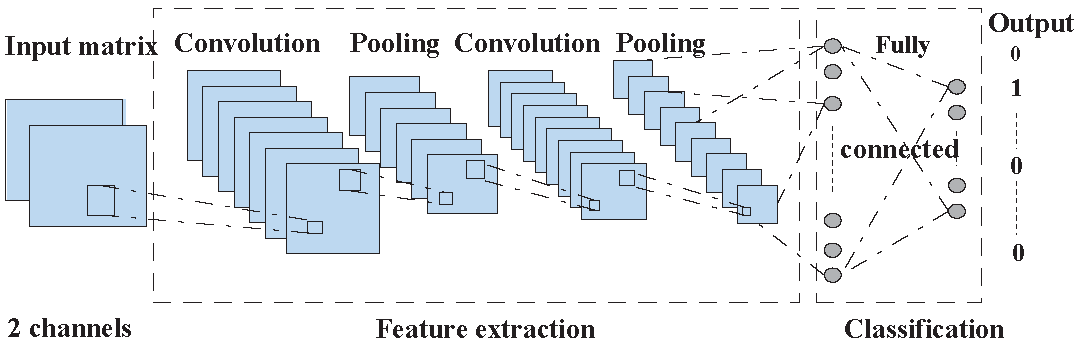
\includegraphics[width=1\textwidth]{a.png}
\end{minipage}
}
\subfigure[input characterization]{
\begin{minipage}[b]{0.5\textwidth}
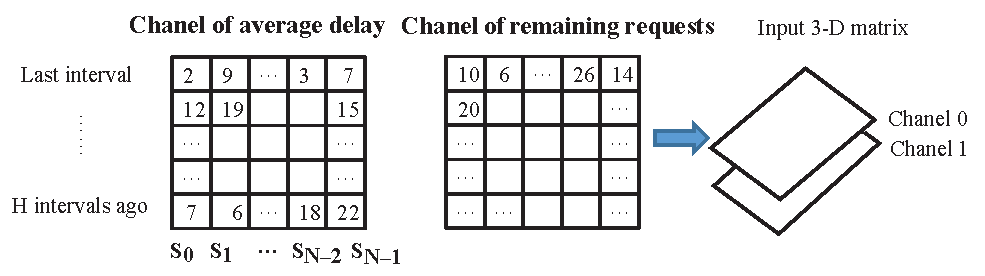
\includegraphics[width=1\textwidth]{b.png}
\end{minipage}
}
 \caption{Our input characterization for the deep CNN} 
 \label{fig:label}
\end{figure}

\subsubsection{Initialization Phase}
As described in Input and Output Design, we need labeled data to train our CNN model. In the initialization phase, we need to obtain the labeled data. The purpose of the initialization phase is to get the labeled data which consist of the input vector and the corresponding output result. It is best to train our CNN model with the global solution of formula 12. However, the time complexity of solving the optimal solution is $O(n^m)$, which is not tolerated. We choose a compromised method to get the labeled data. We adopt a heuristic algorithm to obtain the near-optimal solution.  As shown in algorithm 2, the simulated annealing(SA) algorithm mainly consists of two key step: generate a new solution with some functions and accept the new solution with a certain probability. We take the solution of our greedy algorithm as the initial solution in SA algorithm.

The SA algorithm iterates $L$ times at a certain temperature to search the global optimal solution. In the searching process, the SA algorithm poor solution with the probability of $\exp(-\frac{\triangle t}{T})$, where $\Delta t$ is the evaluation difference between the new solution and the origin. With the SA algorithm, we can obtain the labeled data for our CNN model. The input of our CNN model is the records information of servers in last $H$ intervals. Thus, we obtain the record information of servers and the corresponding offloading result.

\begin{algorithm}[!h]   
\caption{Simulated Annealing Algorithm}   
\label{alg:Framwork}   
\begin{algorithmic}[1]
\REQUIRE ~~\\ %算法的输入参数:Input  
The set of requests  $\mathit{Q}=\left\{q_1,q_2,\dots,q_m \right\} $;\\  
The list of servers $S=\left\{s_1,s_2,s_3,\dots,s_n \right\}$;\\ 
The tolerable total delay $D$ \\
\ENSURE ~~\\
The minimum of power consumption ;\\
The serial number of server nodes for requests \\ 
\STATE Initial temperature T,temperature threshold $T^{'}$, iterations L
\STATE Initial solution\\ $s \leftarrow Greedy  Algorithm(Q,S,D)$
\WHILE{$T>T'$}
\REPEAT
\STATE  Displace some requests from high performance to low performance randomly
\IF{Delay<D}
\STATE Get new solution $s'$
\ENDIF
\STATE calculate $\Delta t = C(s')-C(s)$
\IF{random [0,1] < $\mathrm{e^{\frac{-\Delta t}{T}}}$}
\STATE accept new solution $s'$
\STATE record serial\_list,$C(s')$
\ENDIF
\IF{satisfy final condition}
\RETURN $C(s')$, serial\_list
\ENDIF
\STATE$K \leftarrow K+1$
\UNTIL{K==L}
\STATE $T = \alpha\cdot T$, where $\alpha$ is an attenuation factor
\ENDWHILE
\RETURN $C(s')$, serial\_list
\end{algorithmic}  
\end{algorithm}  
\subsubsection{Training Phase}
In the training phase, we use the data obtained in initialization phase to train the CNN model. The training phase consists of two step: initializing the parameters in our designed CNN and fine-tuning the parameters with BP(back-propagation) algorithm. It is necessary to initial the parameters,which is benefit to accelerate the convergence speed. The CNN parameters are initialized by normal Gauss distribution with a mean value of zero. 

For feed-forward neural network, parameter optimization depends on the error back-propagation. The optimization phase can be done by the stochastic gradient descent(SGD) algorithm or the Adam algorithm. Since the Adam algorithm is adaptive, we choose adam as the optimization algorithm in our training phase as shown in Algorithm 3. In the training phase, we take the cross-entropy cost function as the loss function. Thus, the output is a scalar which is the neuron index of the maximum value in the output layer.
\begin{algorithm}[!h]   
\caption{Training Algorithm}   
\label{alg:Framwork}   
\begin{algorithmic}[1]
\REQUIRE ~~\\
$(x,y)= \left\{(x^{(t)},y^{(t)})|t=1,2,\dots,m \right\}$
\ENSURE  ~~\\
$\theta$
\STATE initial $\theta$ randomly
\FOR{$(x_i,y_i) \in (x,y)$}
\STATE predict = forward($x_i$,$\theta$)
\STATE loss = loss\_fun(predict,$y_i$)
\STATE loss.backward()
\STATE update $\theta$
\ENDFOR
\end{algorithmic}  
\end{algorithm} 

\subsubsection{Running Phase} 
In running phase all servers need to record the number of received requests and average power consumption over a period of time and send these records to edge computing nodes. In this way, each edge node can take these records as an input to calculate the offloading result. However, it is possible to obtain an inappropriate result which doesn't meet the constraints in the CNN running phase. In such situation, we take the greedy algorithm as an compensation.


\section{PERFORMANCE EVALUATION}
In order to validate the performance of our model, we conduct the simulations on the front end and back end. The related parameters in the simulation is shown as table 2.
\begin{table}[h]
	\centering
	\begin{tabular}{p{3cm}p{3cm}}
	\hline
	Variable & Value \\\hline   
	$N$             & 20\\
	$M$             & 5\\
	$n_j$           & $20\sim25$ \\
	$f_i$           & $4.5\sim5.5$ \\
	$f_j$           & $2.5\sim3.5$ \\
	request packet size & $5\sim15MB$ \\
	request need cycles & $0.7\sim0.9$ \\\hline
	\end{tabular}
	\caption{parameters}
\end{table}

As mentioned before, we used the predictive combination-mode model in the front-end. Before sending requests, broadcast packets are sent to ask the nearby vehicles or RSU for the back-end processing delay. With the delay result and vehicle speed, vehicles can calculate the arriving RSU when the requst returns. In the combined-model, the power consumption and delay of V2I,V2V model are estimated to choose the optimal model. In the simulation, we assume that vehicles are travelling in a straight line and the simulation result is shown as figure 3

\begin{figure}[ht] 
  \centering 
  \subfigure[house]{ 
    %\label{fig:subfig:a} %% label for first subfigure 
    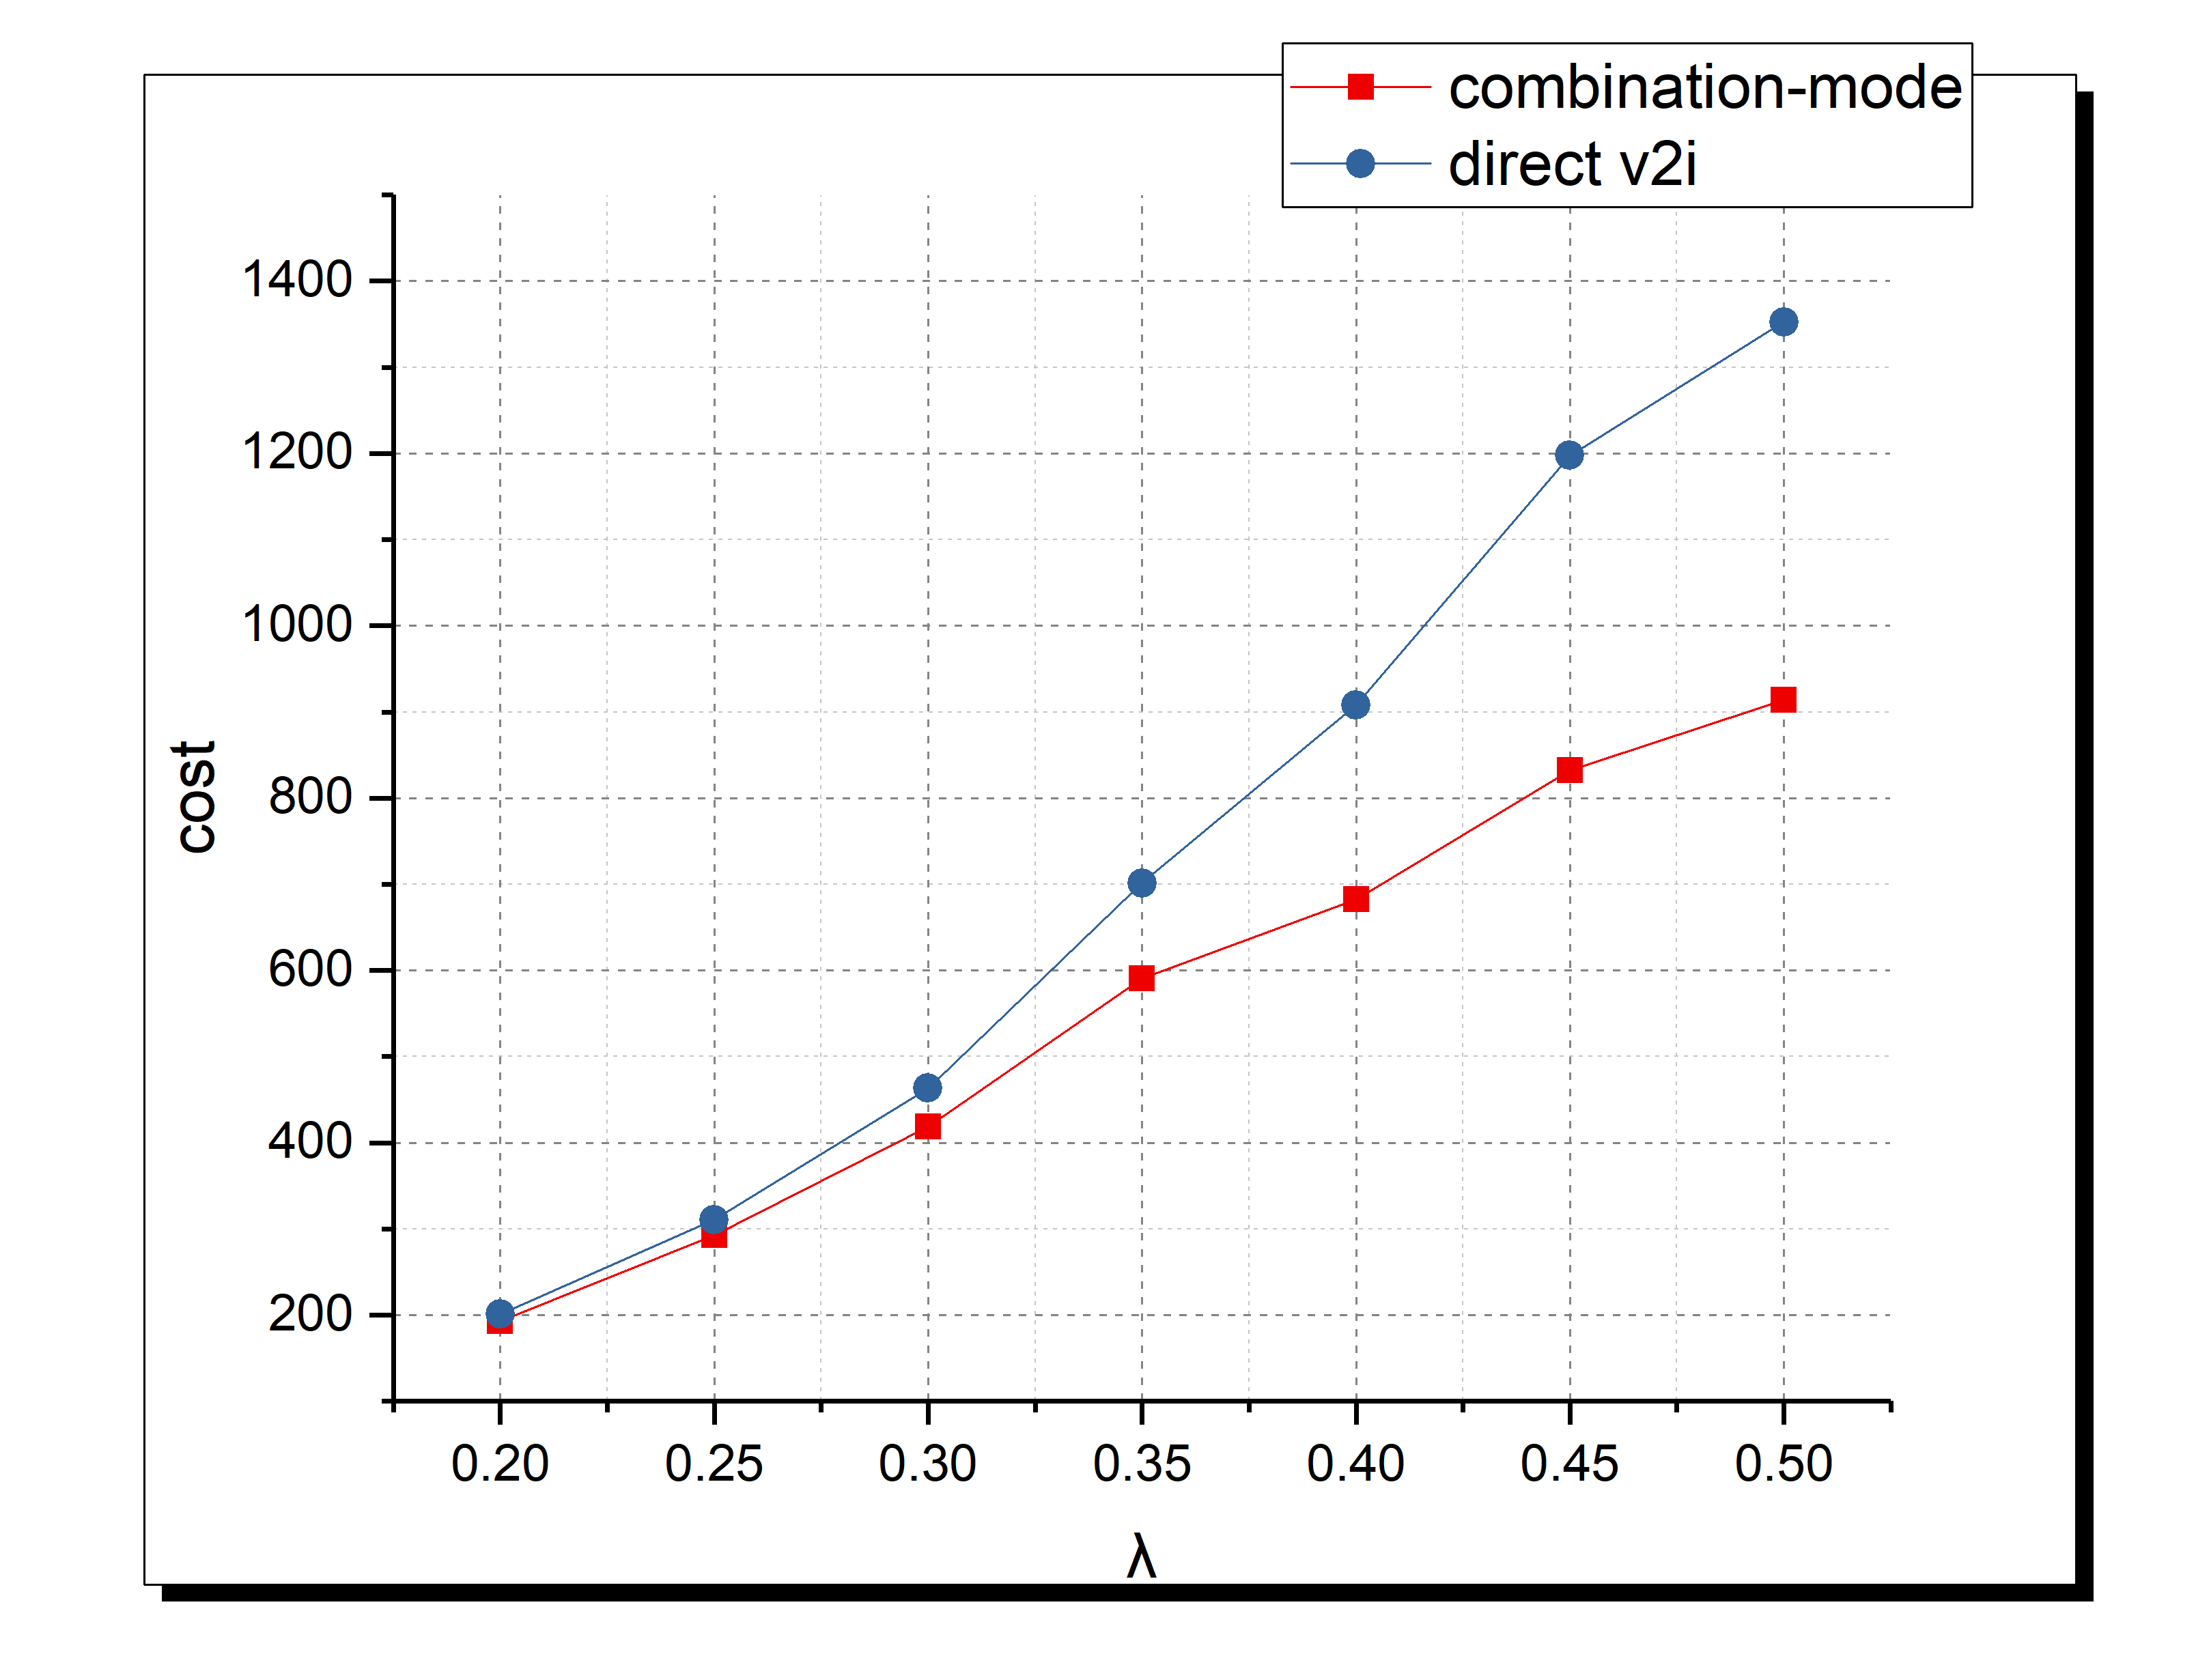
\includegraphics[width=0.22\textwidth]{./c.png} 
  } 
  \subfigure[hotel]{ 
    %\label{fig:subfig:b} %% label for second subfigure 
    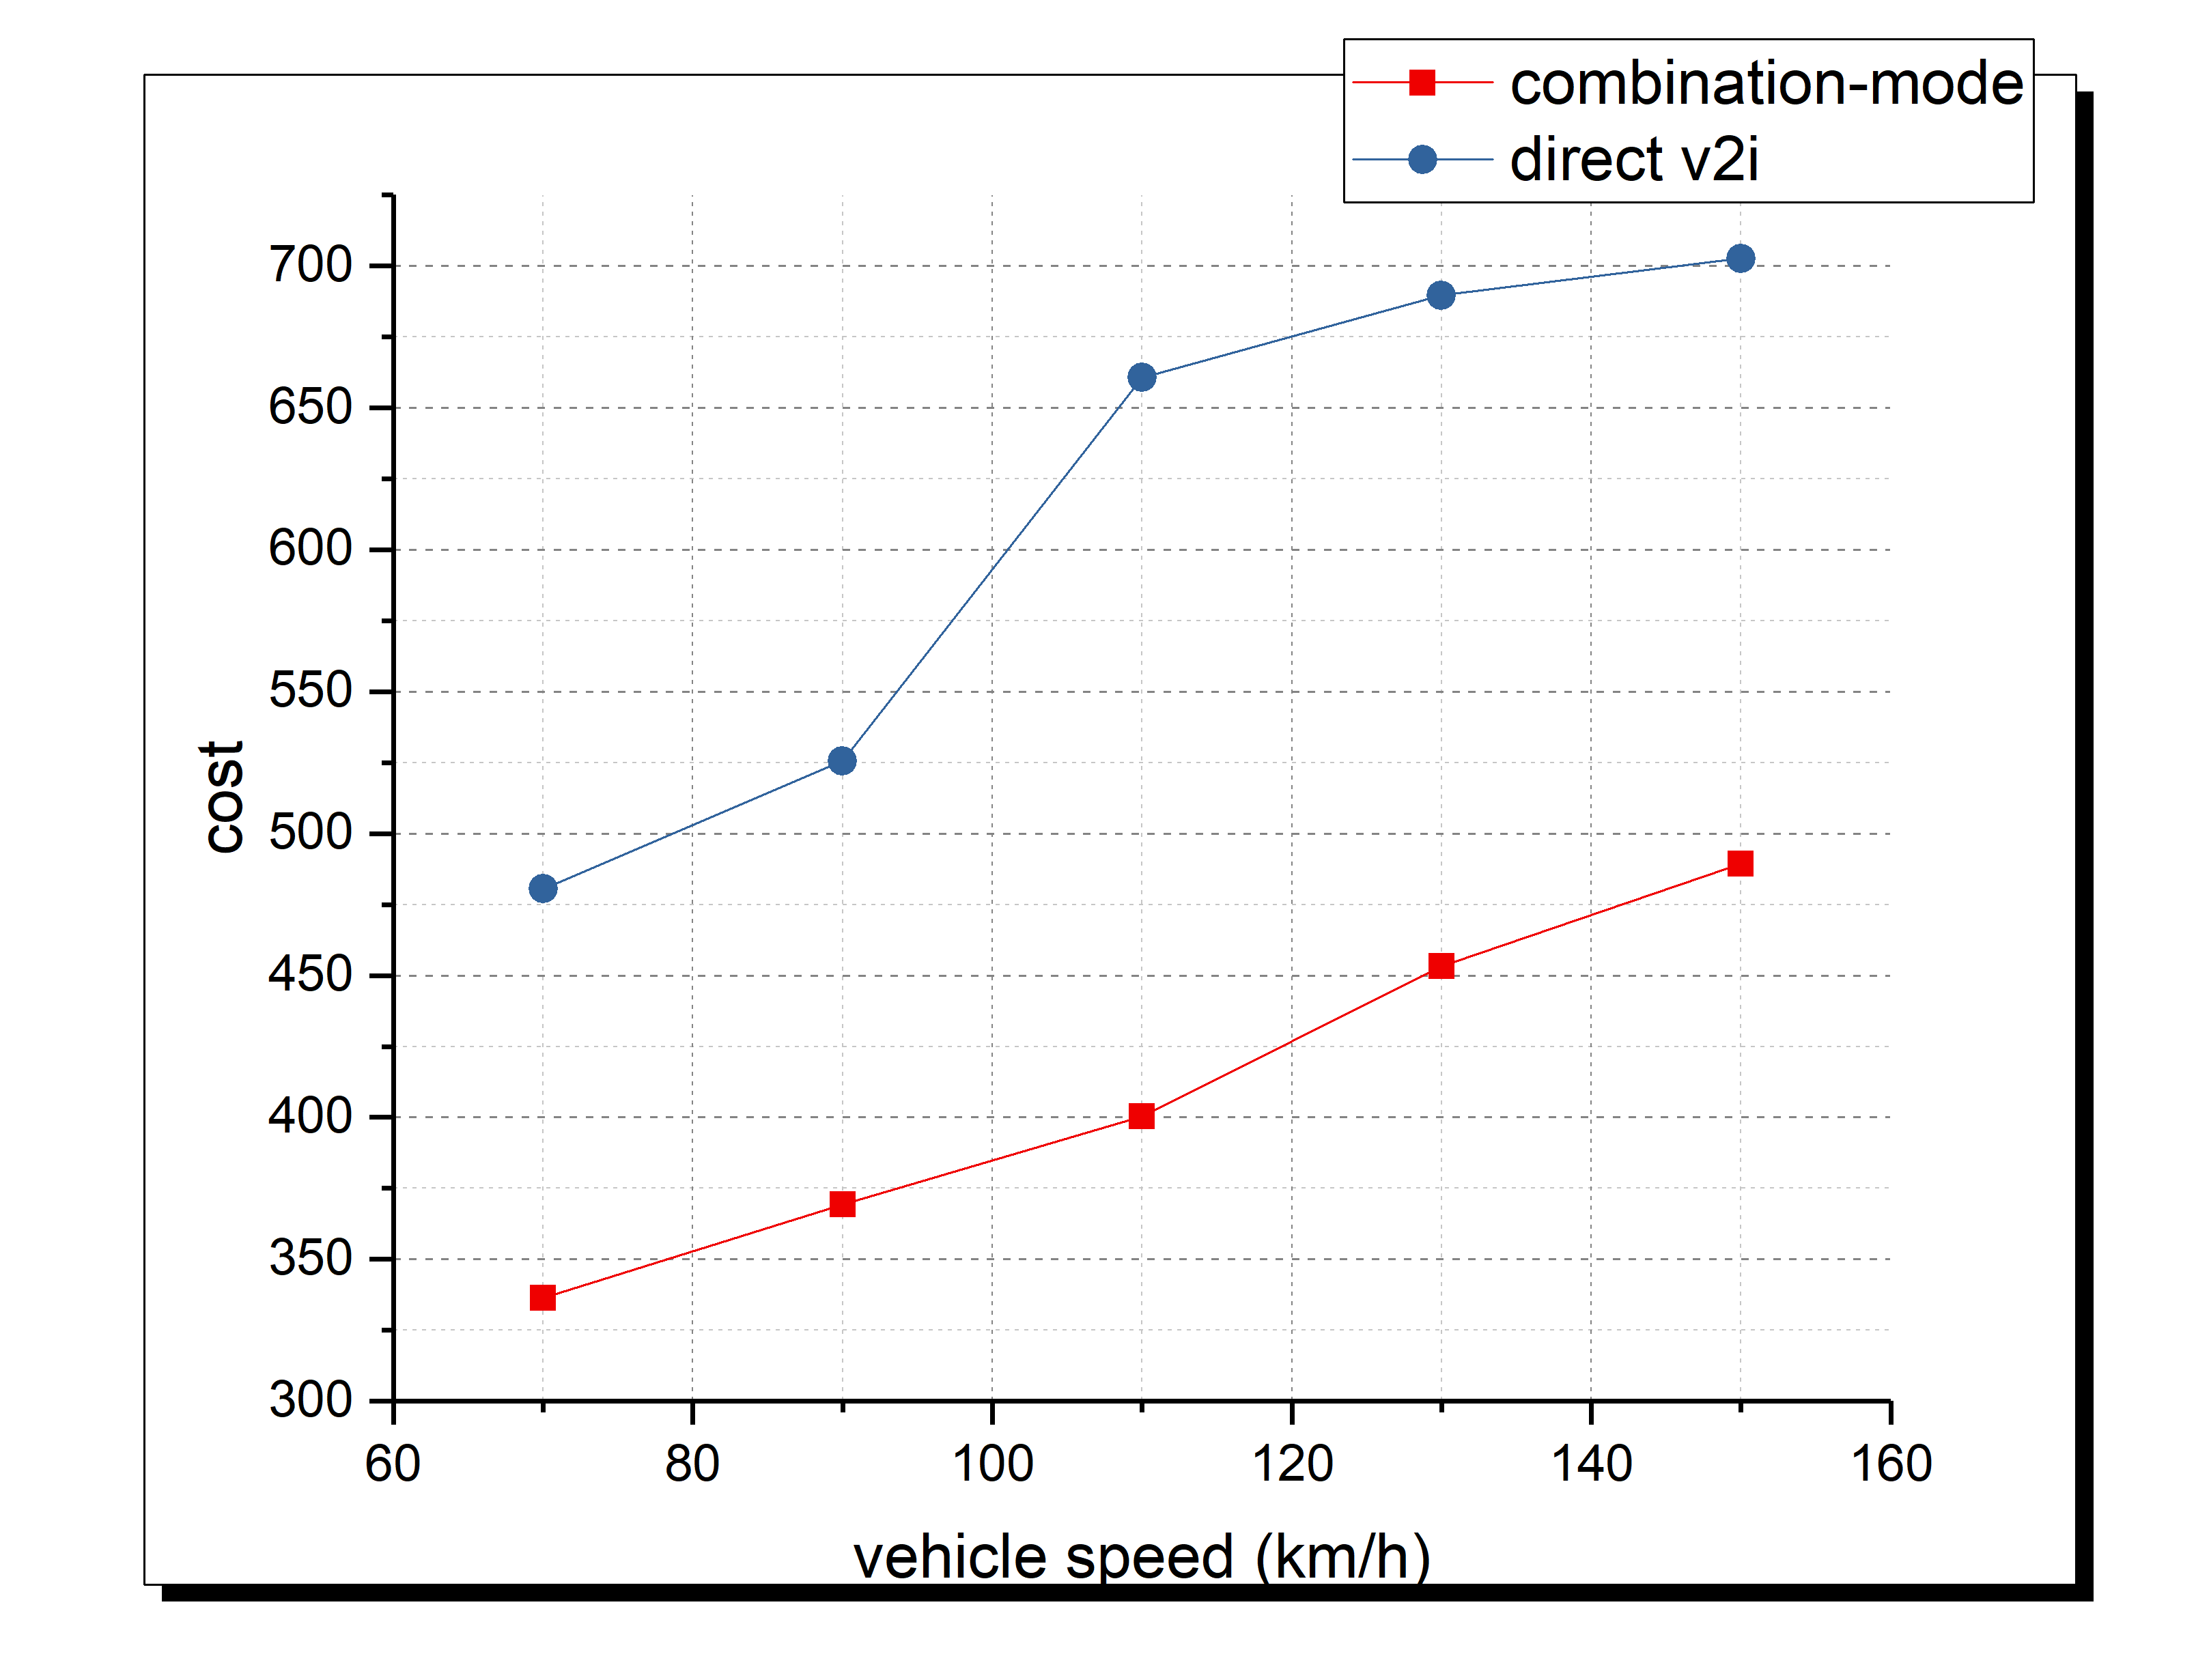
\includegraphics[width=0.22\textwidth]{./d.png} 
  } 
  \caption{} 
  %\label{fig:subfig} %% label for entire figure 
\end{figure}

Figure 3 illustrates the performance of cost with different vehicle speed and vehicle density. With higher vehicle speed, the cost of the combined-mode is much lower than the V2I mode. For the V2I mode, the cost grows significantly with the speed of 100 to 120. That is because with that speed most vehicles are at the edge of RSU coverage when the request returns. Therefore, when the speed exceeds a threshold, the vehicles will drive into another RSU. The cost of V2I mode will increase significantly. In addition, the optimization effect of combined-mode is obvious with a heavy traffic density. With a heavy traffic density, the delay and power consumption of each hop in V2V mode reduced a lot. 

In order to validate the performance of fog-cloud model. We compare the performance of fog-cloud model with cloud-only and fog-only mode. 
\begin{figure}[htp]
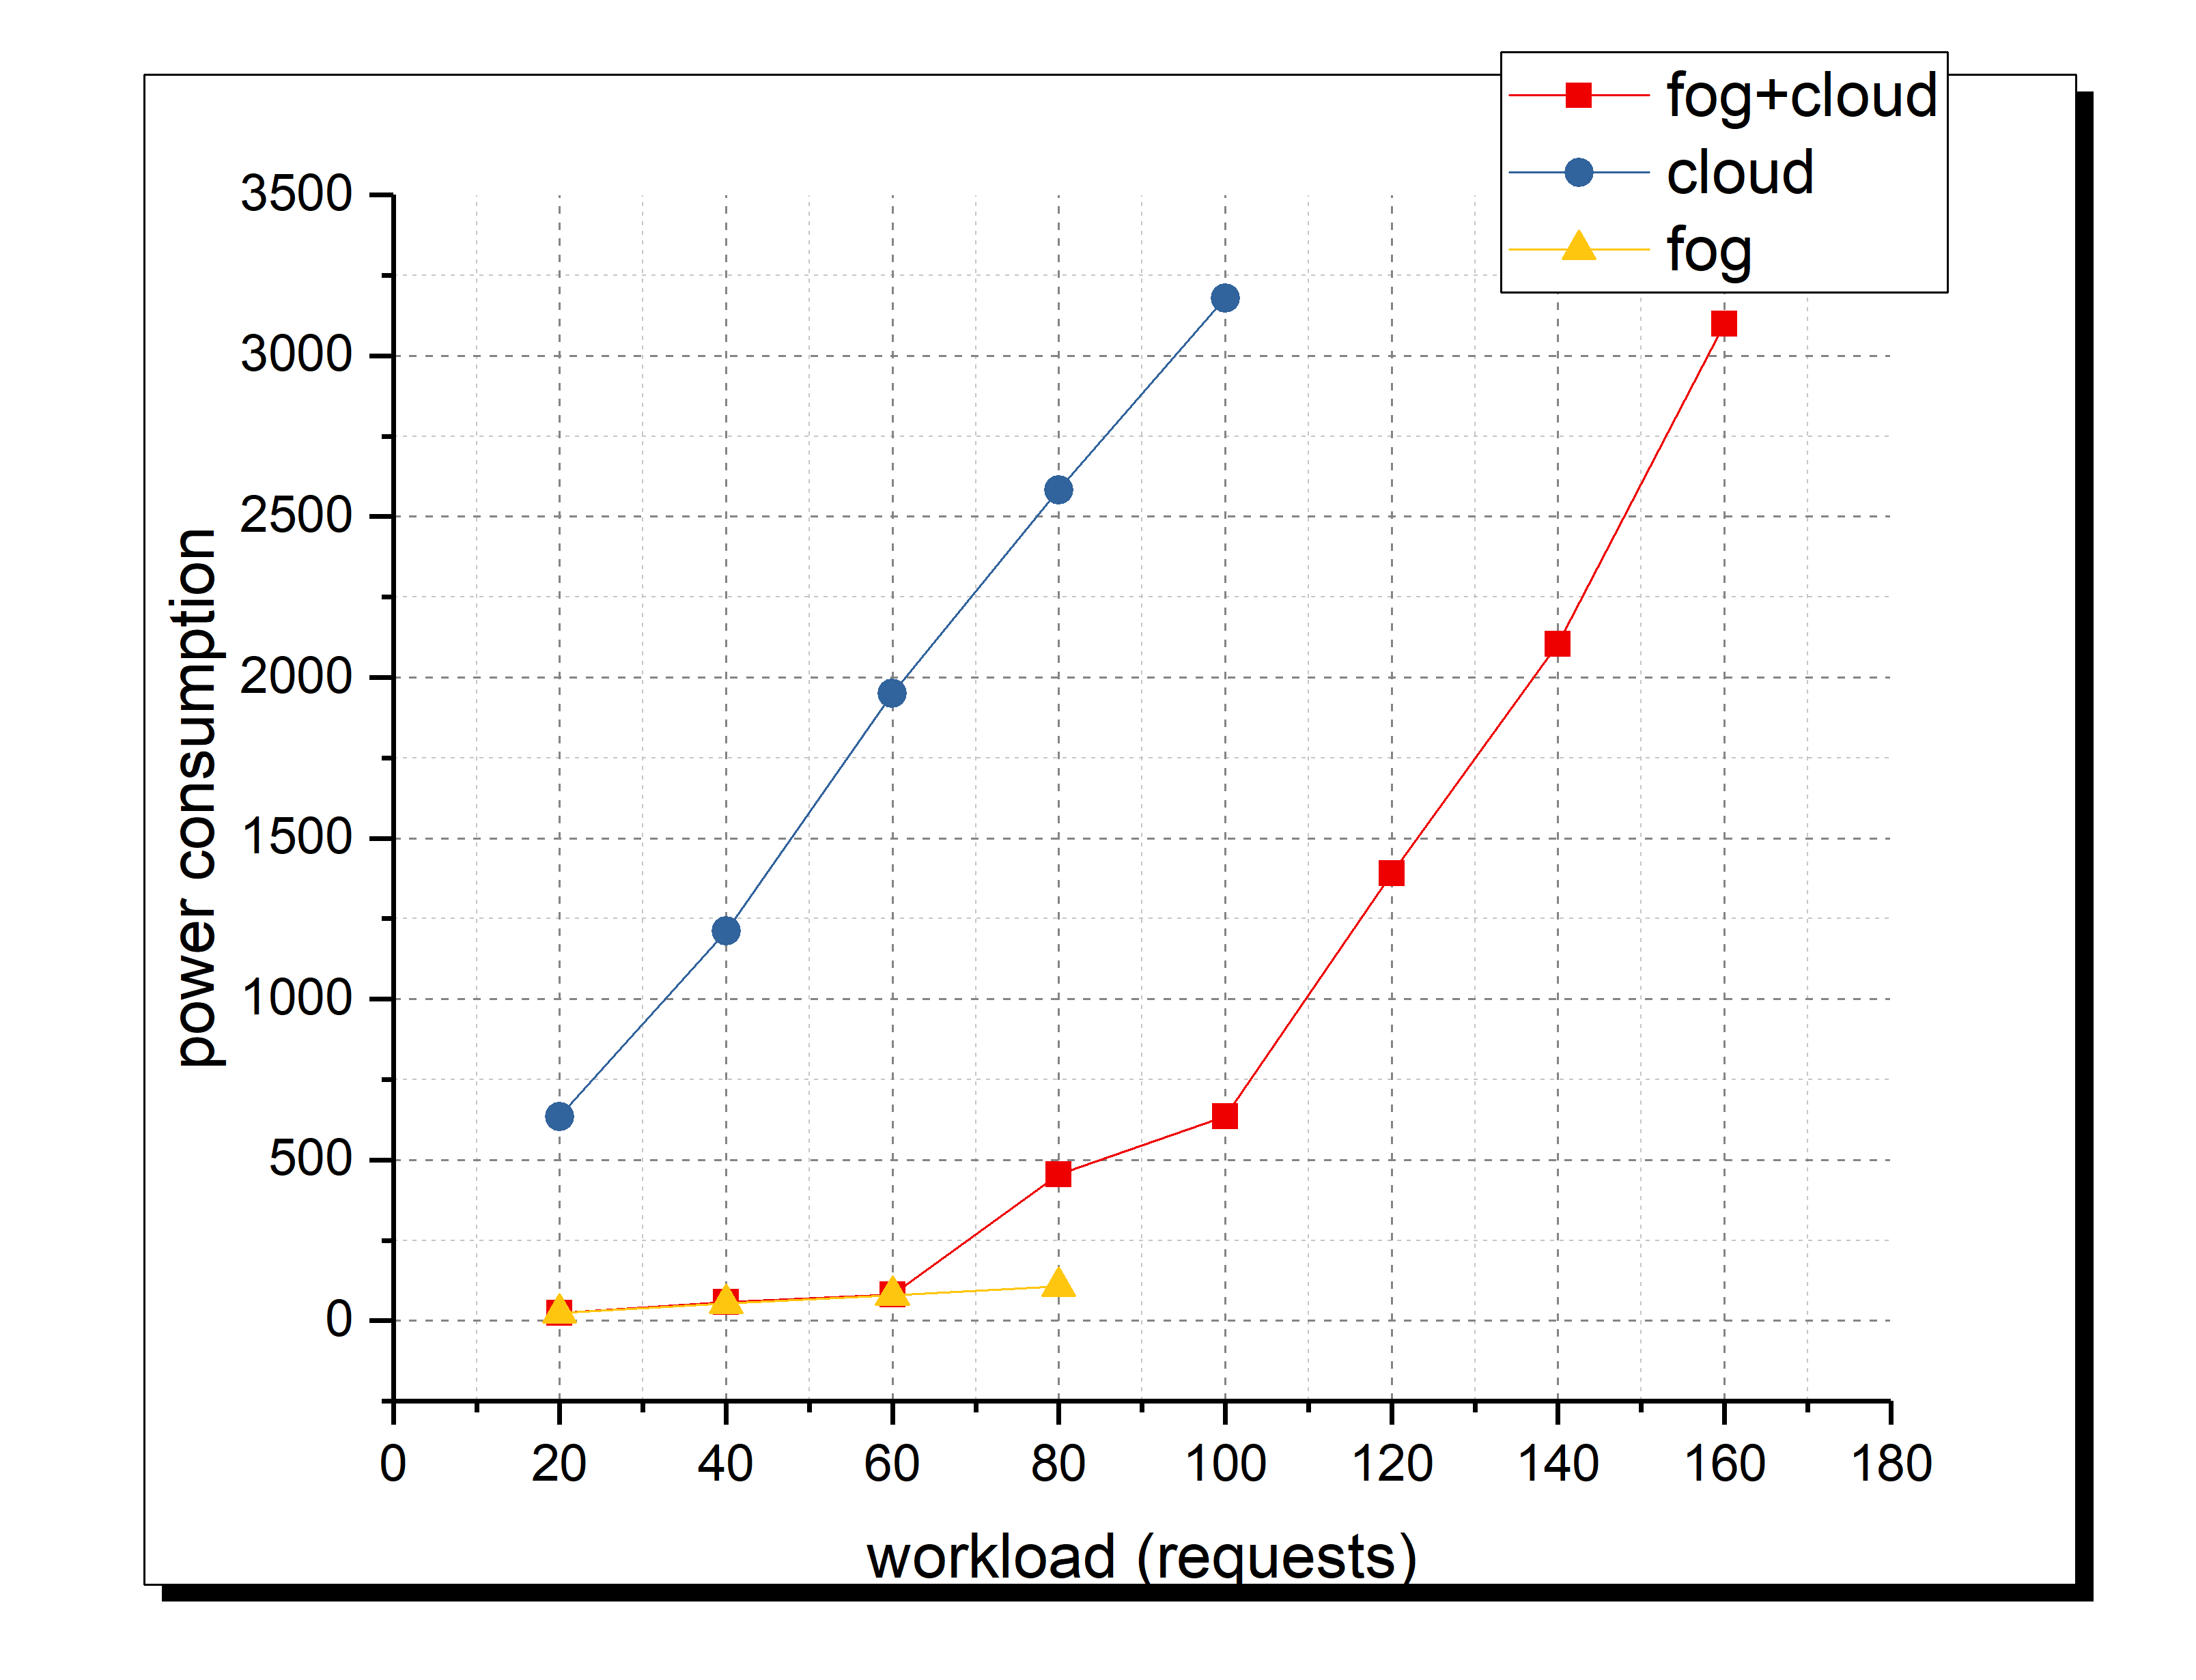
\includegraphics[width = 0.5\textwidth]{e.png}
\caption{Comparison of energy consumption}
\end{figure}

As shown in figure 4, the power consumption of fog-only is extremely low but no more than 80 requests can be handled at one time. The fog-cloud model is much better than the cloud-only model with the workload of 20 to 100. The power consumption of the fog-cloud model is almost the same as that of fog-only model with the workload of 20 to 80. In such situation, the workload of fog layer is not saturated and most requests are processed by the fog node. When the workload is more than 100, the fog layer reaches saturation,after which the power consumption growth trend in the fog-cloud model is similar to the cloud-only model.

Moreover, the maximum workload of fog-cloud model is much larger than the other two models. Figure 5 illustrates the performance of delay with different workload. The average delay of fog-cloud model is less than 1.5 seconds. Whereas, in the other two model the average delay is fast-growing. 
\begin{figure}[htbp]
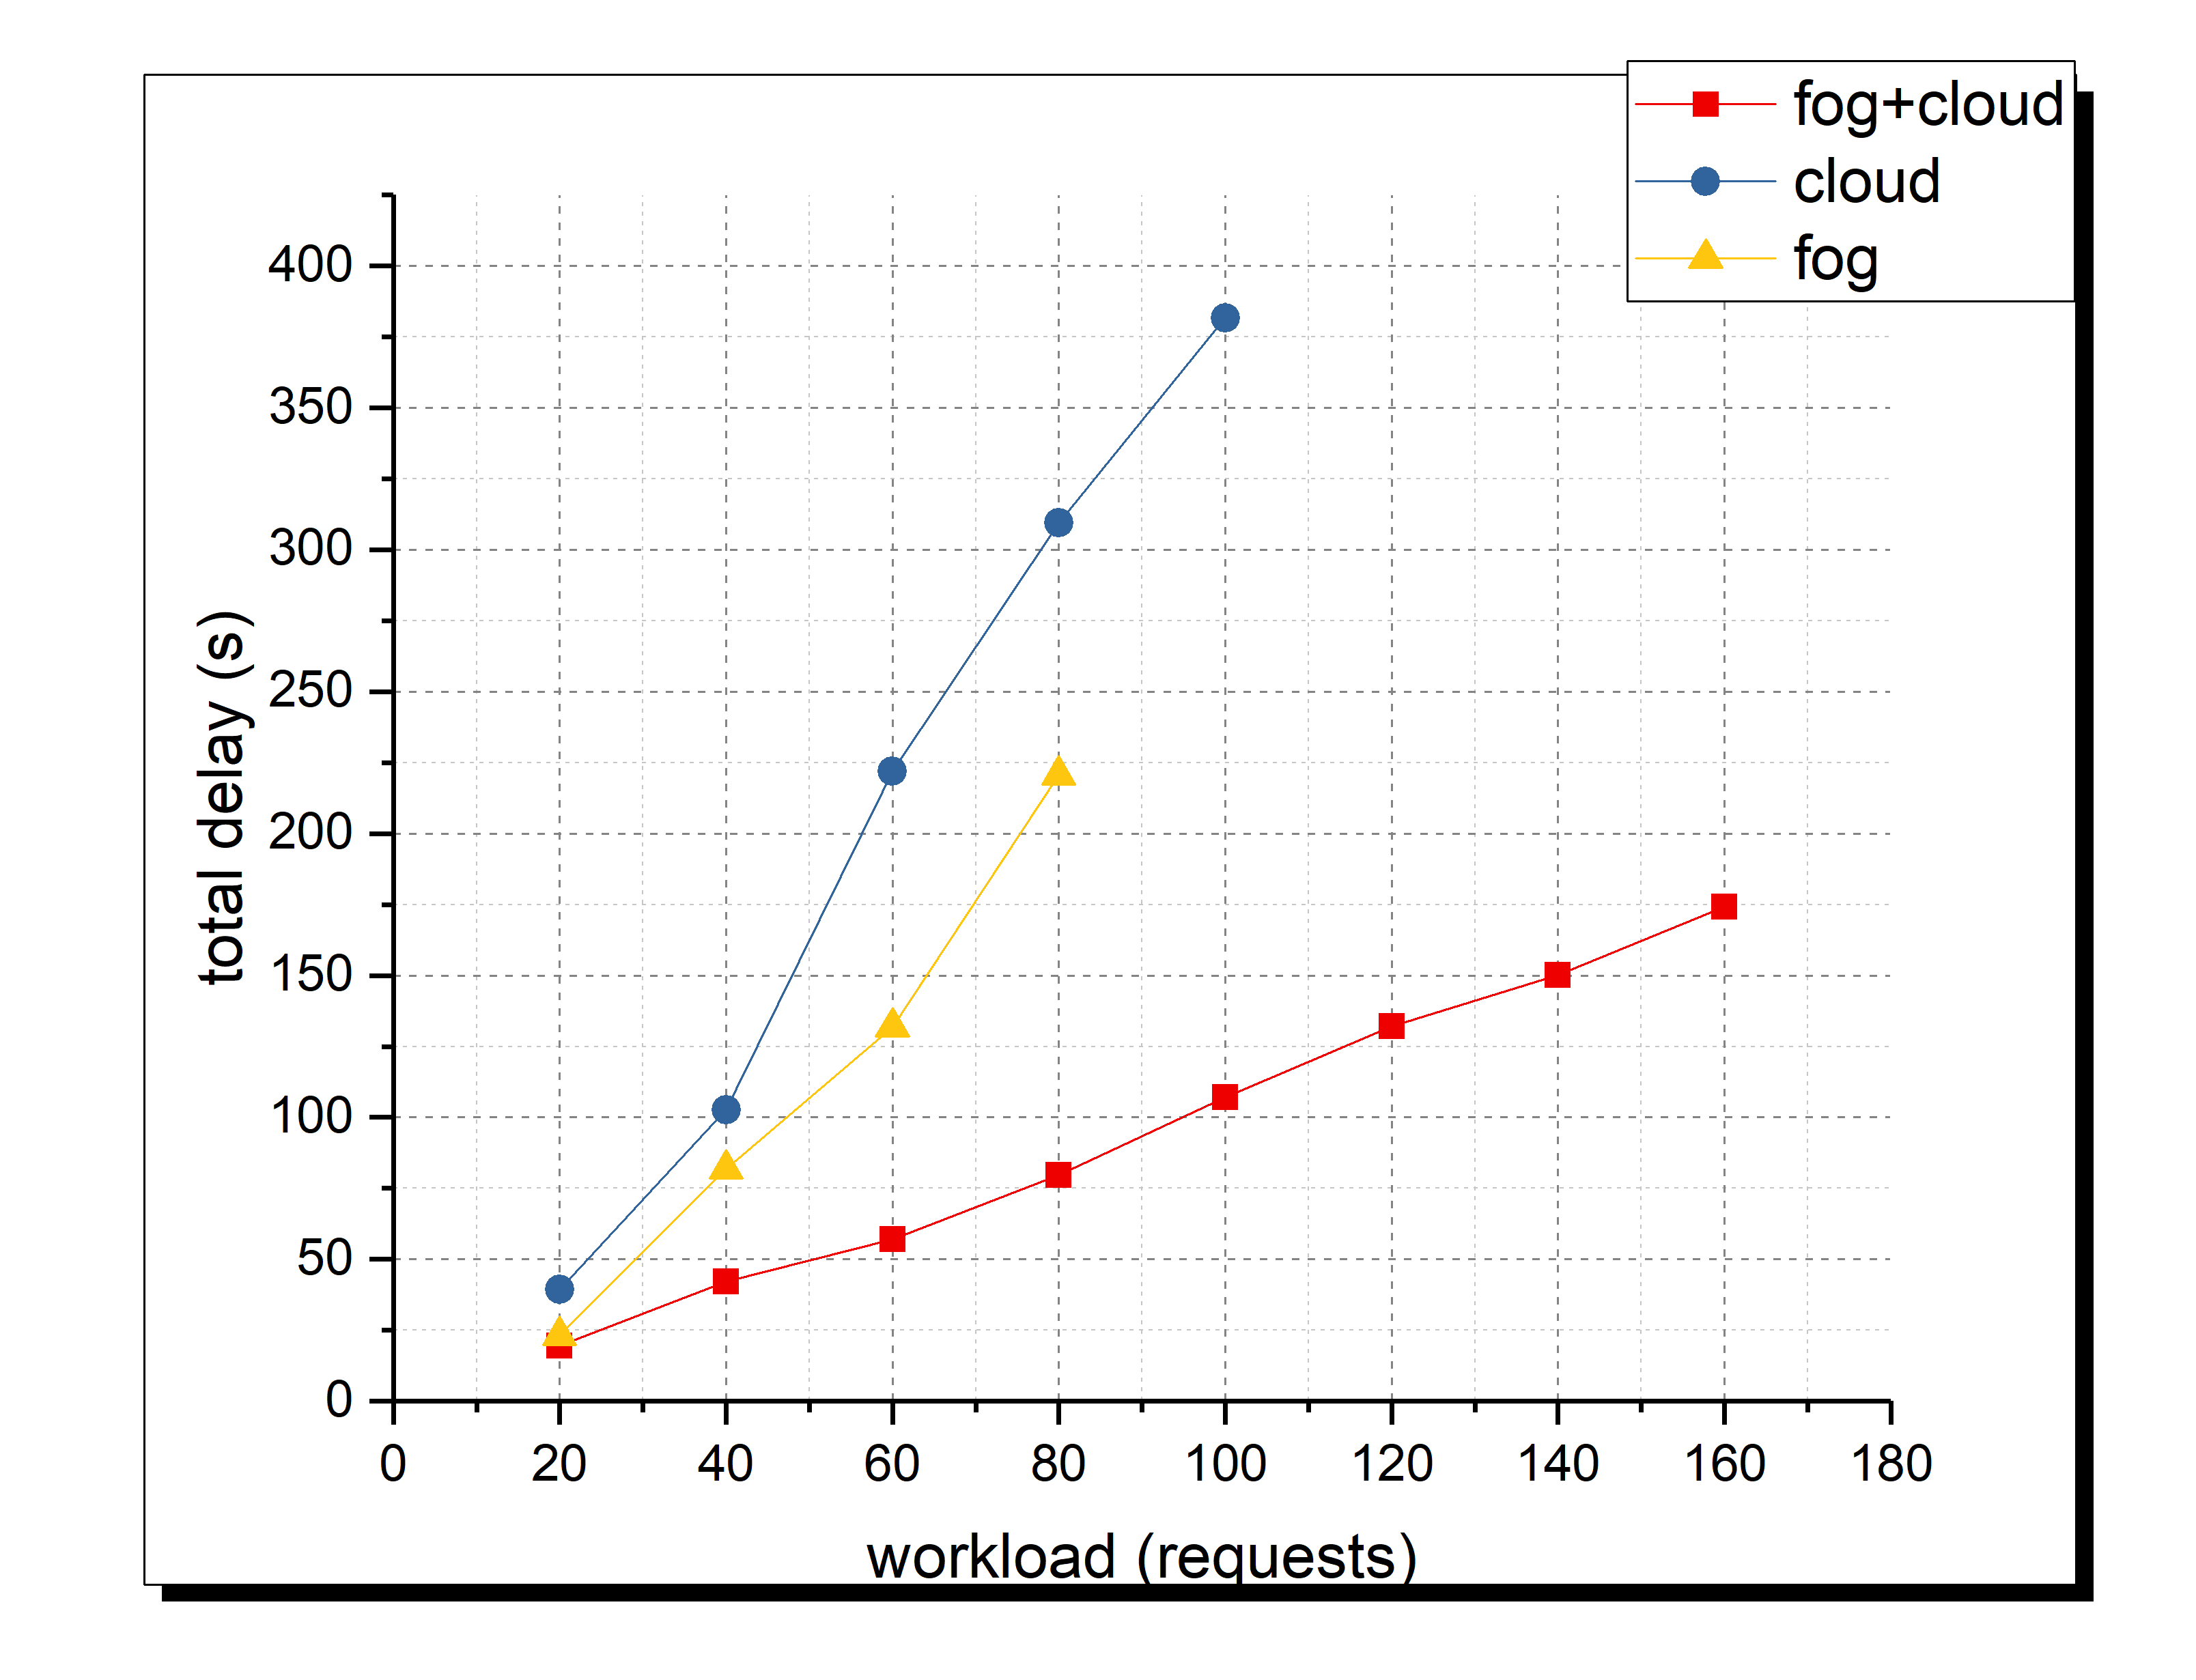
\includegraphics[width = 0.5\textwidth]{f.png}
\caption{Comparison of delay}
\end{figure}

As mentioned before, we take the last H interval records of servers as input in CNN model. The CNN model in the simulation is shown in figure 6. We take the records of last four $\Delta t$ intervals as input, where $\Delta t$ is equal to 2 seconds. In each interval $\Delta t$, the average number of request is 50. The training data is obtained by SA algorithm in 20 consecutive intervals. 
\begin{figure}[htbp]
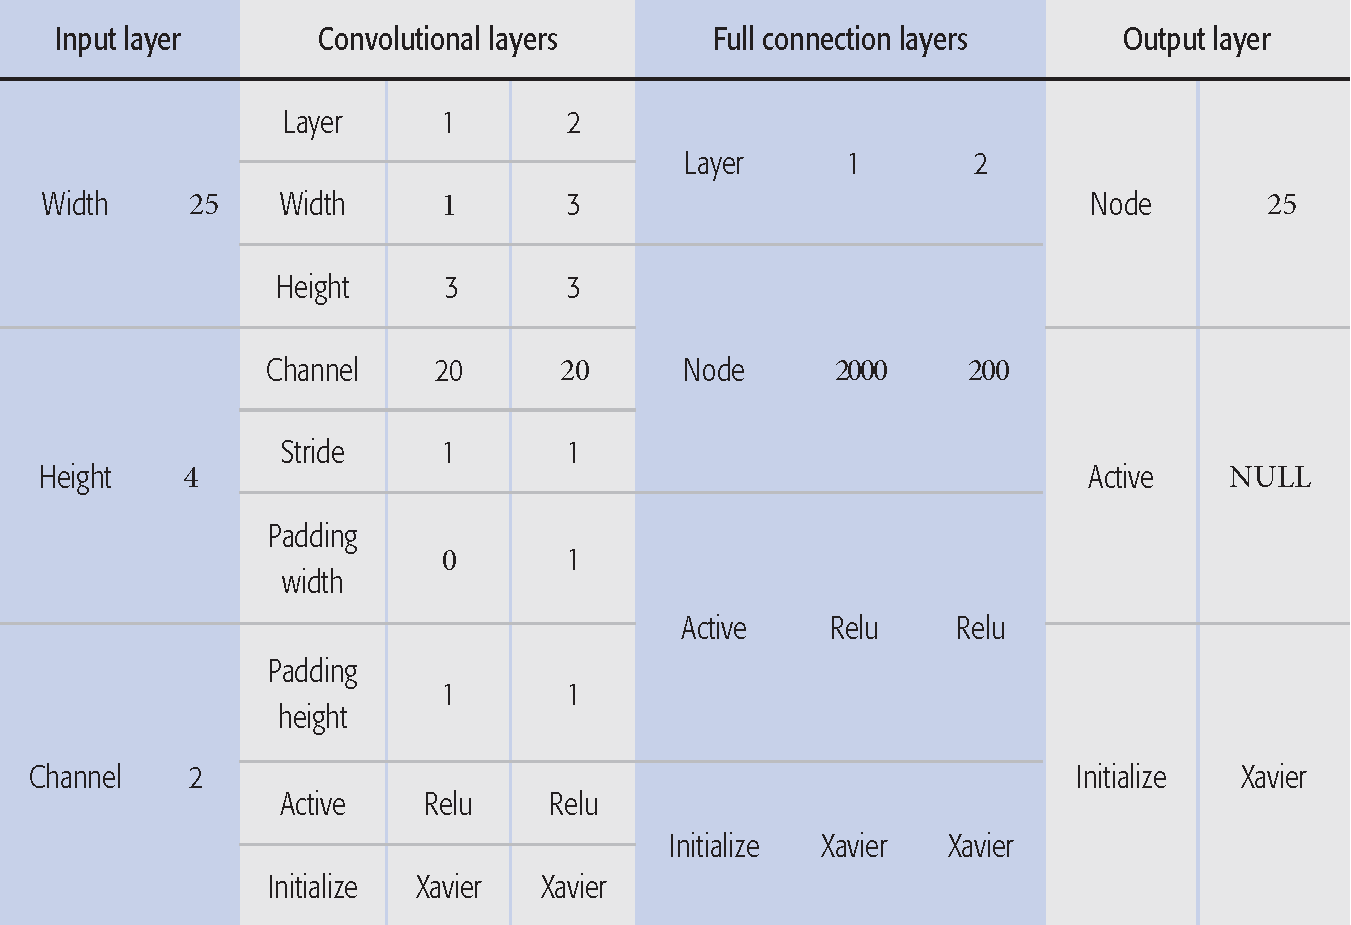
\includegraphics[width = 0.5\textwidth]{g.png}
\caption{CNN model structure}
\end{figure}

After training, we obtain the offloading result of requests by CNN model. The power consumption of different algorithm is shown in figure 7. Our deep learning model can effectively reduce the computational complexity in the running phase and the performance is much better than the greedy algorithm
\begin{figure}[htbp]
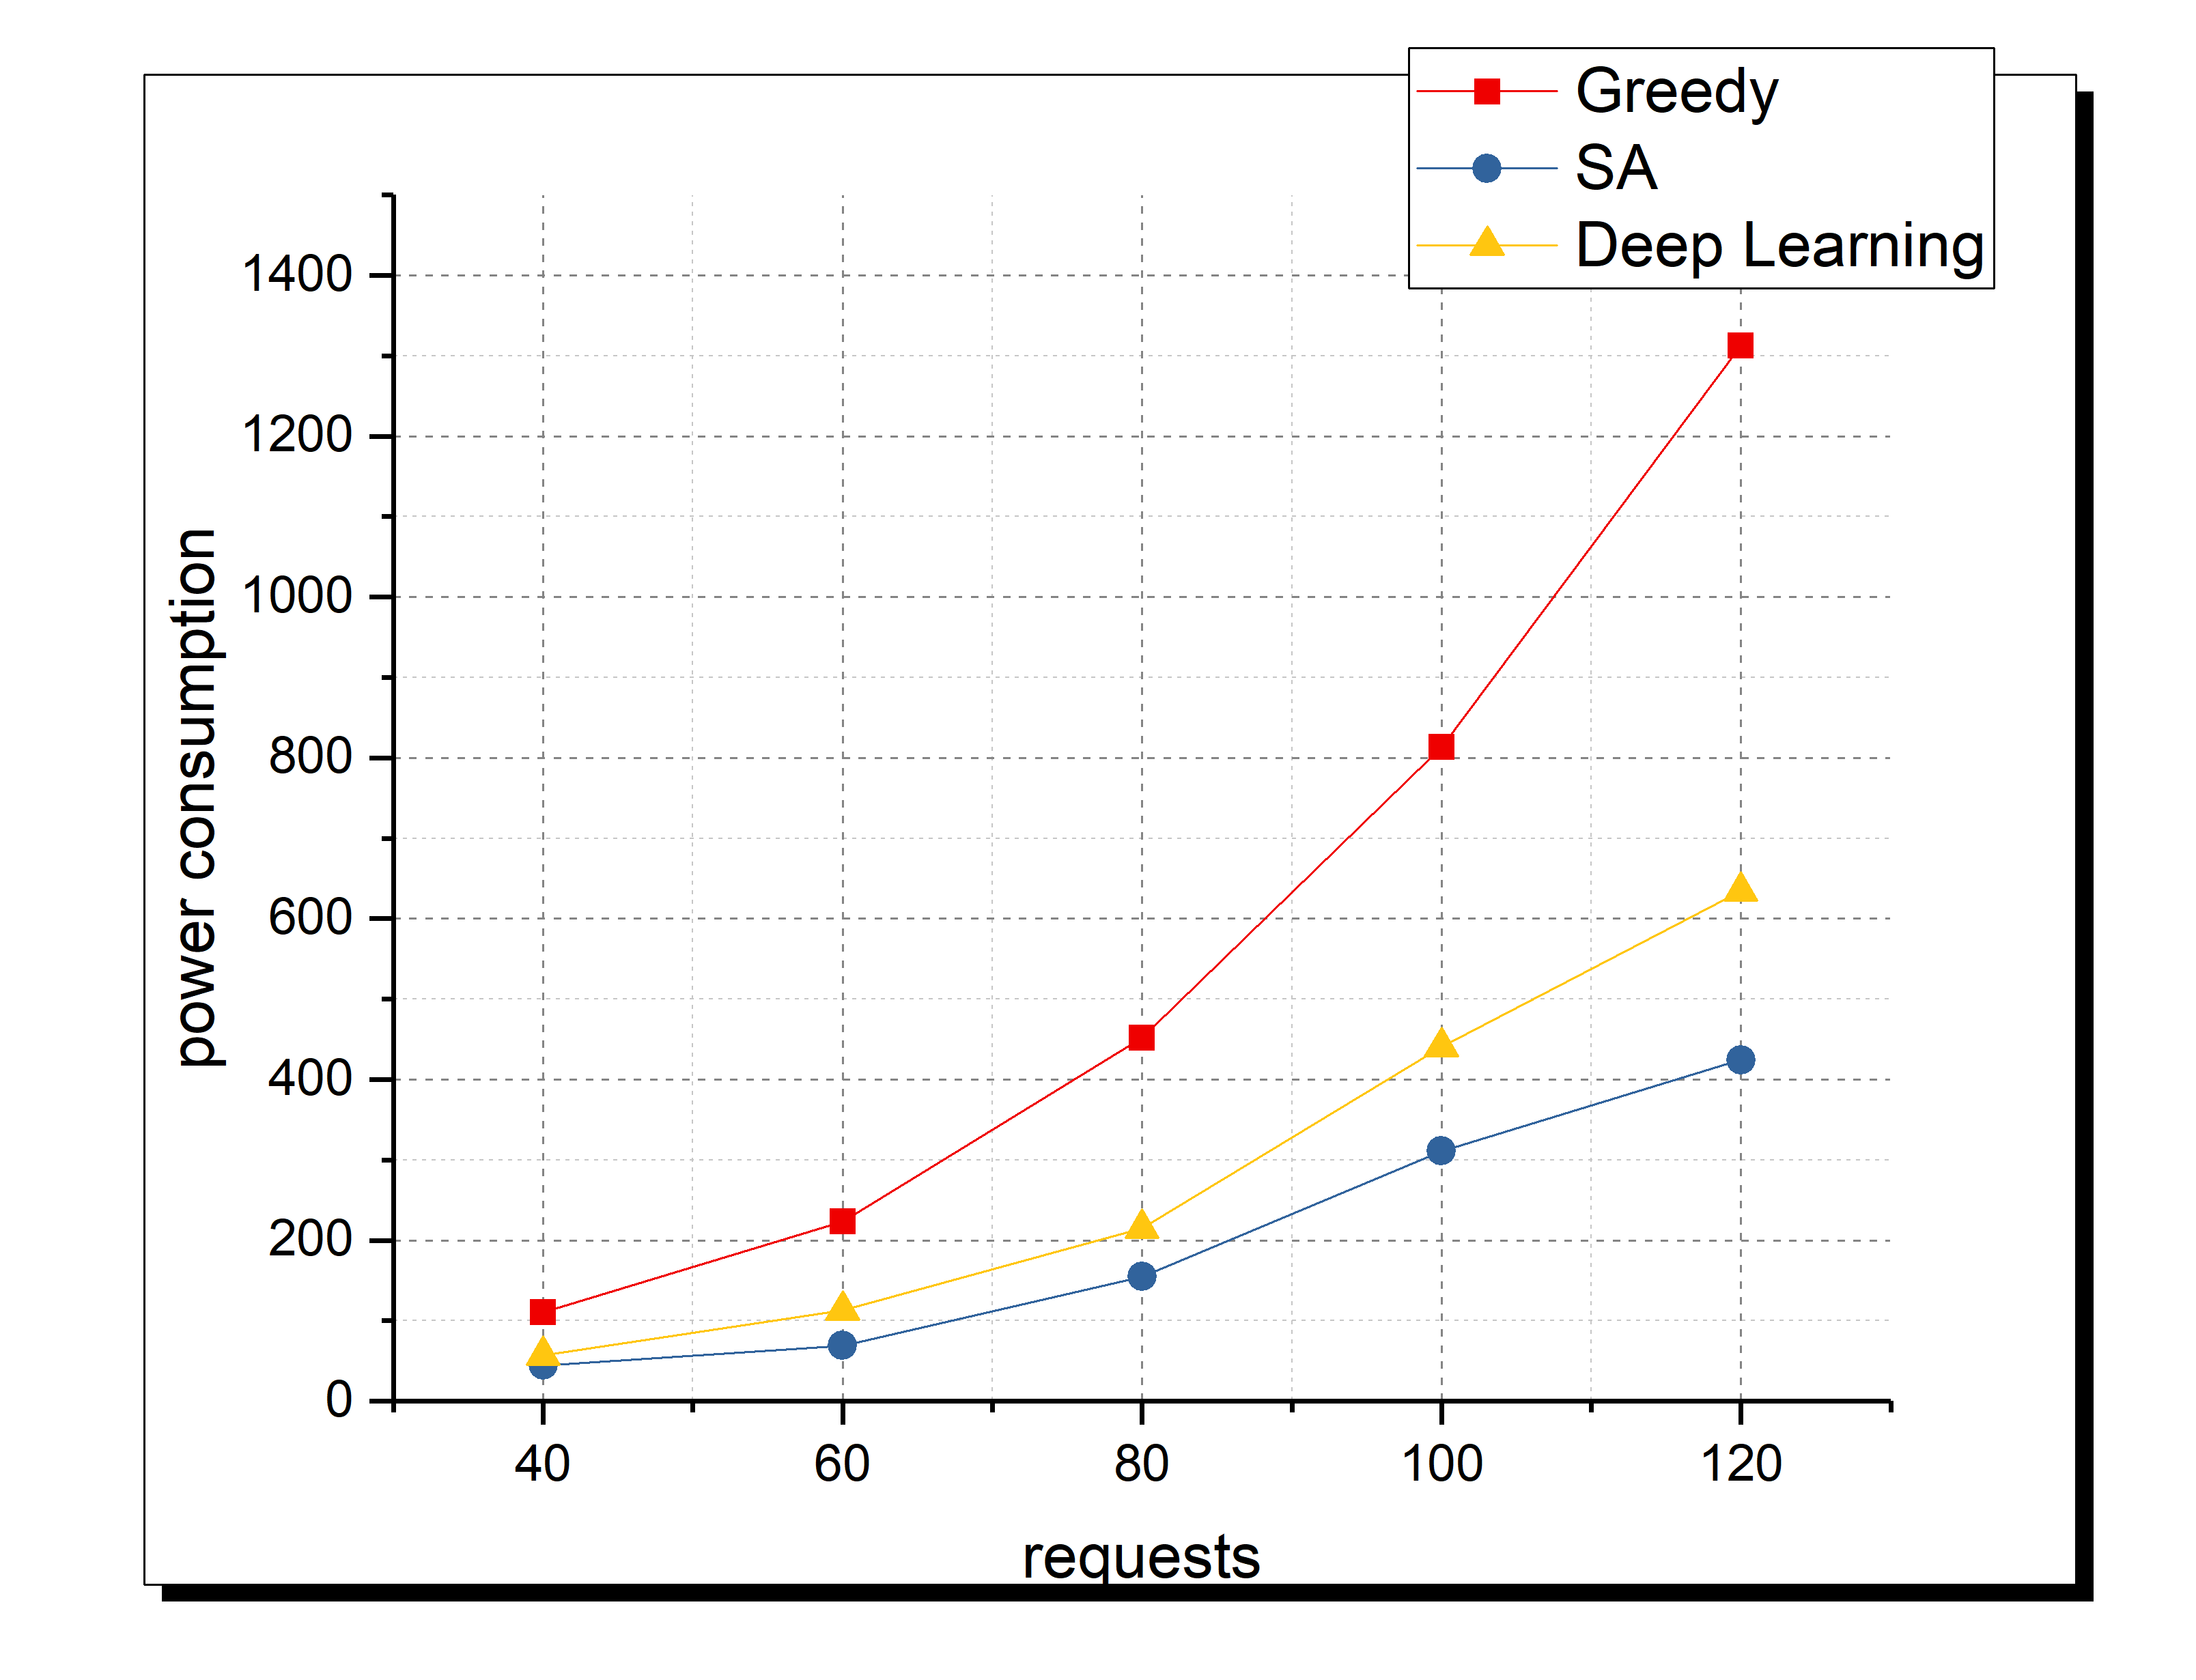
\includegraphics[width = 0.5\textwidth]{h.png}
\caption{Power Consumption of Deep Learning and other algorithm}
\end{figure}


\section{Conclusion}
In this paper,we propose a fog-cloud model based on deep learning ,which is a feasible solution to minimize the power consumption and delay in the back-end. The offloading optimization problem is formulated in our proposed model.For the fog nodes, they can be modeled as M/M/1 in queueing theory. For the cloud servers, they can be modeled as M/M/n queue. In addition, we propose a predictive combination-mode model to minimize the cost in front-end. In the simulation, we can draw the conclusion that the fog-cloud model shows good performance compared to the cloud-only mode or the fog-only mode. Our deep learning model is an approximate approach to solved the formulated problem.
%\bibliographystyle{plain}
%\bibliography{lunwen}
\end{document}
